\section{Resultados}
A rede neural auto-organizável implementada nesse trabalho, utilizou o algoritmo Mapa de Kohonen, desenvolvido por
Teuvo Kohonen em 1982 \cite{}. Para os resultados práticos, a rede foi treinada com um conjunto de 1728 exemplos de dados 
reais, fornecidos pelo site \textit{UCI Machine Learning Repository}\footnote{http://archive.ics.uci.edu/ml/}, variando
valores da taxa de aprendizado, pesos iniciais, raio da vizinhança e quantidade de neurônios na rede. O conjunto de exemplos 
escolhido foi o \textit{Car Evaluation}\footnote{http://archive.ics.uci.edu/ml/datasets/Car+Evaluation}, onde dados os 
atributos preço de compra do veículo, custo da manutenção, quantidade de portas do veículo, número de passageiros, tamanho do
bagageiro e segurança estimada do veículo, avalia se o veículo é aceitável, inaceitável, bom ou muito bom. Uma vez que o 
algoritmo Mapa de Kohonen organiza ou agrupa dimensionalmente os dados, o conjunto de exemplos foi adaptado, 
apresentando somente três dimensões (preço de compra do veículo, custo da manutenção e segurança estimada do veículo).

\subsection{25 neurônios}
Os gráficos a seguir mostram a plotação dos pontos após a execução do algoritmo para alguns valores de parâmetros e para 
uma rede com 25 neurônios. Apesar de não se poder afirmar se o algoritmo convergiu, vemos que aumentando o raio de vizinhança,
o algoritmo consegue ``especializar'' melhor o conjunto. O efeito da taxa de aprendizado está sobre a velocidade na qual o 
algoritmo irá convergir. Ela geralmente é dada empiricamente, assim como os pesos iniciais, que segundo \cite{}, se forem
inicializados com valores iguais, faz o algoritmo convergir mais rapidamente.

\begin{figure}[ht!]
	\centering
	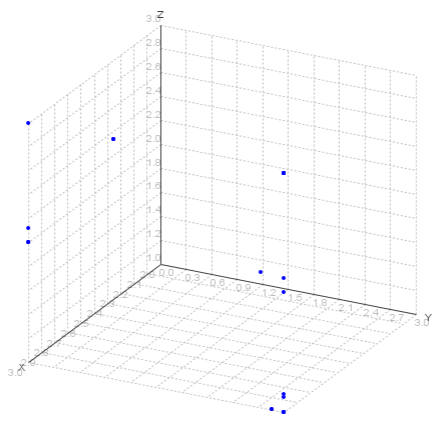
\includegraphics[scale=0.65]{./imgs/2a1.png}
	\caption{Taxa de aprendizado: 0.8662815917277779; Raio: 1; Pesos iniciais: A}
\end{figure}

\begin{figure}[ht!]
	\centering
	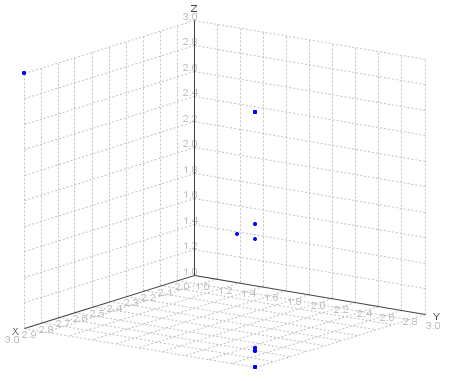
\includegraphics[scale=0.65]{./imgs/2a2.png}
	\caption{Taxa de aprendizado: 0.8662815917277779; Raio: 2; Pesos iniciais: A}
\end{figure}

\begin{figure}[ht!]
	\centering
	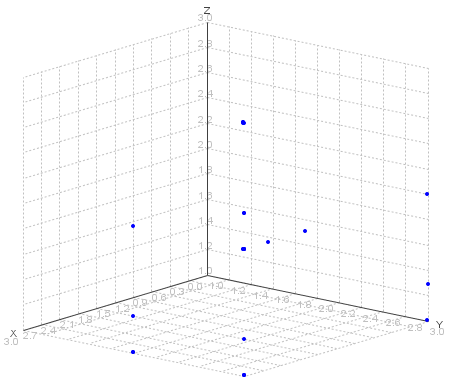
\includegraphics[scale=0.65]{./imgs/2b1.png}
	\caption{Taxa de aprendizado: 0.5980629675758204; Raio: 1; Pesos iniciais: B}
\end{figure}

\begin{figure}[ht!]
	\centering
	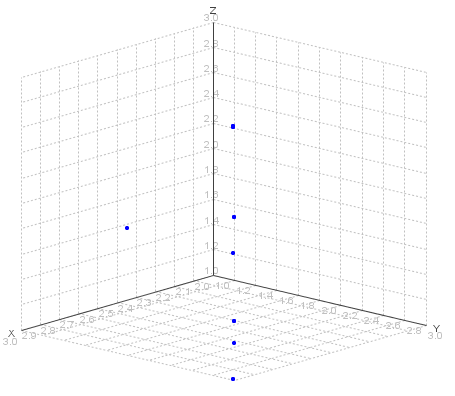
\includegraphics[scale=0.65]{./imgs/2b2.png}
	\caption{Taxa de aprendizado: 0.5980629675758204; Raio: 2; Pesos iniciais: B}
\end{figure}

\subsection{36 neurônios}
Os gráficos a seguir mostram a plotação dos pontos após a execução do algoritmo para alguns valores de parâmetros e para
uma rede com 36 neurônios.

\begin{figure}[ht!]
	\centering
	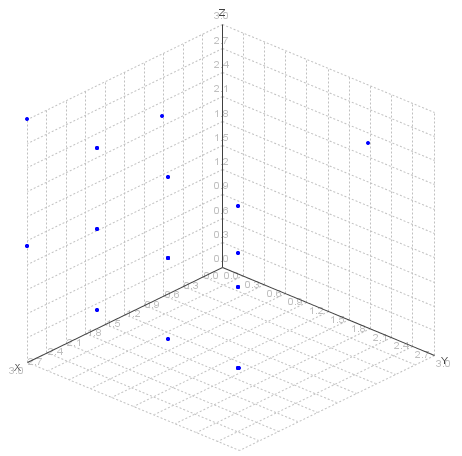
\includegraphics[scale=0.65]{./imgs/2d1.png}
	\caption{Taxa de aprendizado: 0.2625656059885696; Raio: 1; Pesos iniciais: D}
\end{figure}

\begin{figure}[ht!]
	\centering
	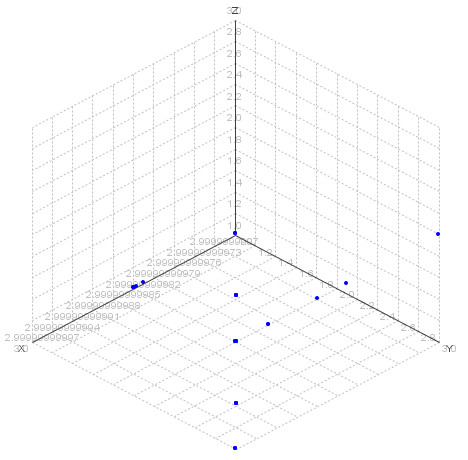
\includegraphics[scale=0.65]{./imgs/2d2.png}
	\caption{Taxa de aprendizado: 0.2625656059885696; Raio: 2; Pesos iniciais: D}
\end{figure}

\begin{figure}[ht!]
	\centering
	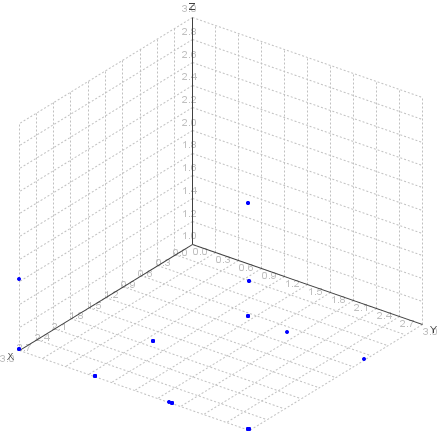
\includegraphics[scale=0.65]{./imgs/2e1.png}
	\caption{Taxa de aprendizado: 0.5517820314689292; Raio: 1; Pesos iniciais: E}
\end{figure}

\newpage
\begin{figure}[ht!]
	\centering
	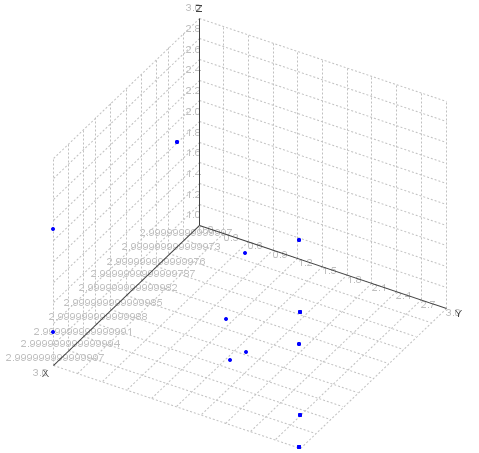
\includegraphics[scale=0.65]{./imgs/2e2.png}
	\caption{Taxa de aprendizado: 0.5517820314689292; Raio: 2; Pesos iniciais: E}
\end{figure}